\section*{Problema 10}
\textbf{Considera el siguiente grafo:}
\begin{figure}[H]
    \centering
    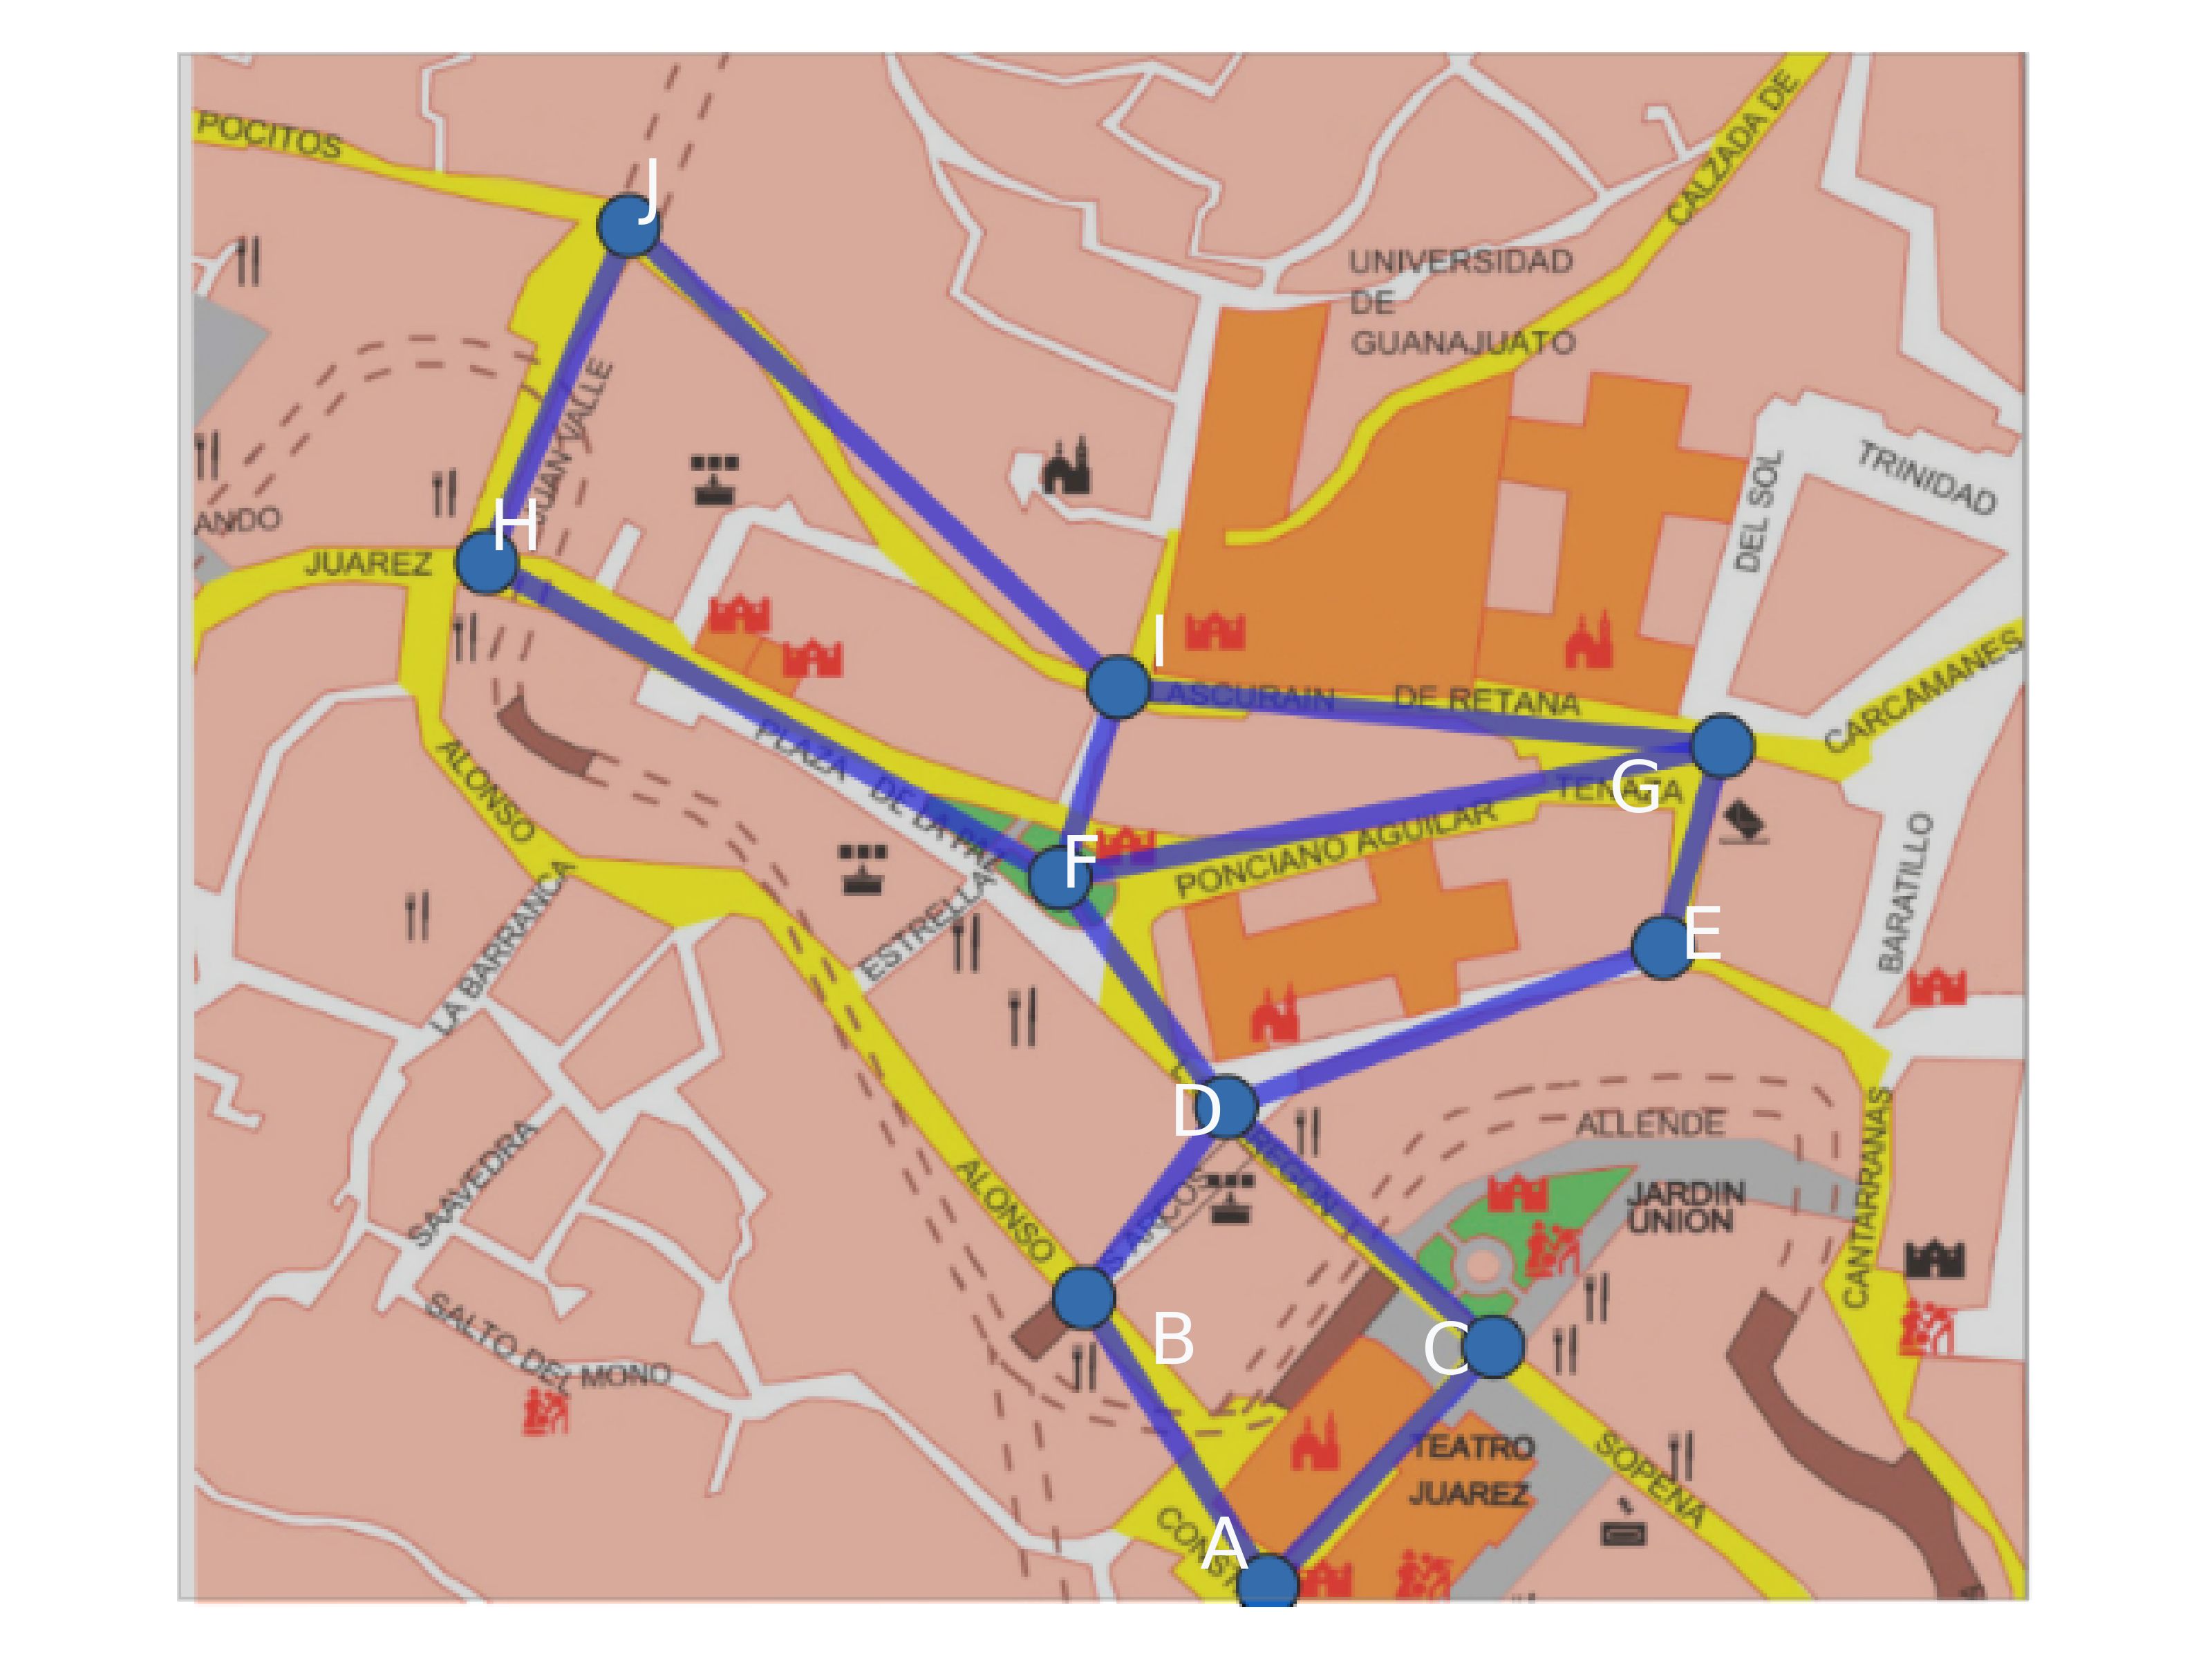
\includegraphics[width=10cm]{Graphics/map.png}
    \caption{Mapa del sitio con los nodos nombrados}
    \label{fig:map_with_letters}
\end{figure}
\textbf{Cada calle (arista) entre dos nodos esté bloqueda por una manifestación con probabilidad p. Supongamos que todos son eventos independientes.}
\subsection*{Problema 10a}
\textbf{Calcula la probalidad de poder caminar desde la puerta trasera del Teatro Juarez (nodo más abajo) al café conquistador (nodo más hacia arriba).}

Llamaremos $P(X_1\rightarrow X_2)$ a la probabilidad de poder caminar desde un nodo $X_1$ hasta un nodo $X_2$ sin repetir nodos intermedios y tomando en cuenta todos los caminos posibles entre $X_1$ y $X_2$.

En la figura \ref{fig:map_with_letters} se muestran los nodos, a los que hemos nombrado $A,B, ..., J$ para mayor simplicidad. Además, llamaremos $p_{\alpha\beta}$ a la probabilidad de que el vértice entre los nodos $\alpha$ y $\beta$ esté libre, es decir que se pueda caminar por la calle que une los dos puntos.
\par A nosotros nos interesa la probabilida de que haya camino libre desde el nodo de más abajo (el nodo $A$) hasta el nodo de más arriba (nodo $J$), es decir, nos interesa $P(A\rightarrow J)$. Si tomamos en cuenta que todos los caminos desde $A$ hasta $J$, pasan por $D$ podemos afirmar lo siguiente:
$$
    P(A\rightarrow J) = P(D\rightarrow J)P(A\rightarrow D)
$$
Es decir, para que se pueda caminar desde $A$ hasta $J$, tiene que haber camino libre entre $A$ y $D$ y entre $D$ y $J$. De la misma manera podemos decir que para que los nodos $D$ y $J$ estén conectados, debe haber paso entre $D$ y $H$ y entre $H$ y $J$, o podemos caminar desde $D$ a $I$ y después de $I$ a $J$. Esto, lo podemos escribir de la siguiente manera:
$$
    P(A\rightarrow J) = \left[p_{HJ}P(D\rightarrow H) + p_{IJ}P(D\rightarrow I)\right]P(A\rightarrow D)
$$
A partir de ahora procederemos a simplificar esta expresión utilizando la misma lógica que en los pasos anteriores:\\ Si necesitamos que los caminos de $X_i$ a $X_j$ y los caminos de $X_j$ a $X_k$ estén desbloqueados, la probabilidad de este evento es el producto de las probabilidades. Y si necesitamos que haya paso de $X_i$ a $X_k$ o de $X_k$ a $X_k$, la probabilidad de este evento, es la suma de las probabilidades.
\begin{align*}
    P(A\rightarrow J) = & \left[p_{HJ}P(D\rightarrow H) + p_{IJ}P(D\rightarrow I)\right]P(A\rightarrow D)                                                                                                 \\
    =                   & \left[ p_{HJ}p_{FH}P(D\rightarrow F)+p_{IJ}P(D\rightarrow I) \right]P(A\rightarrow D)                                                                                           \\
    =                   & \left[ p_{HJ}p_{FH}\left( p_{DF}+p_{GF}p_{EG}p_{DE}+p_{IF}p_{GI}p_{EG}p_{DE} \right)+p_{IJ}\left(p_{FI}P(D\rightarrow F)+p_{GI}P(D\rightarrow G)\right)\right]P(A\rightarrow D) \\
    =                   & [ p_{HJ}p_{FH}\left( p_{DF}+p_{GF}p_{EG}p_{DE}+p_{IF}p_{GI}p_{EG}p_{DE} \right)                                                                                                 \\&+p_{IJ}\left(p_{FI}( p_{DF}+p_{GF}p_{EG}p_{DE} )+p_{GI}( p_{FG}p_{DF}+p_{EG}p_{DE} )\right)]P(A\rightarrow D)\\
\end{align*}
Ahora, notemos que la probabilidad de que una calle está bloqueada es la misma en todos los casos, por lo que podemos simplificar todos los $p_{\alpha\beta}$ haciendo lo siguiente:
$$
    q = p_{\alpha\beta}=1-p\ \forall\alpha, \beta\in\{A,\ B,\ ...,\ J\}
$$
Así, expresión de la probabilidad de que haya camino libre entre $A$ y $J$ se convierte en lo siguiente:
\begin{align*}
    P(A\rightarrow J) =                & \left[ q^2(q+q^3+q^4) +q(q(q+q^3)+q(q^2+q^2))\right]P(A\rightarrow D), \\
    \text{además } P(A\rightarrow D) = & \left[p_{AB}p_{BD}+p_{AC}p_{CD}\right] = 2q^2                          \\
    \text{lo que nos lleva a }         &                                                                        \\
    P(A\rightarrow J) =                & 2q^2\left[ q^3+q^5 + q^6 + q^3+ q^5+ 2q^4\right]                       \\
    =                                  & 2q^8+4q^7+4q^6+4q^5
\end{align*}
Por lo tanto, la probabilidad de poder caminar desde la puerta trasera del Teatro Juarez al café conquistador es:
$$
    P(A\rightarrow J) = 2(1-p)^8+4(1-p)^7+4(1-p)^6+4(1-p)^5
$$
\subsection*{Problema 10b}
\textbf{Decimos que un nodo del grafo está aislado si todas las aristas que llegan (o salen) están bloqueadas. Calcula el promedio del número de nodos aislados.}

Sea i el número de aristas que salen del nodo , $a_i$ el conjunto de  nodos que tienen i aristas y $n_i$ el número de nodos que tienen i aristas. El promedio de nodos aislados puede ser calculado como la suma del promedio de los $a_i$ nodos, entonces:

\begin{align}
    E(A) & = \sum_i E(A_i)     \nonumber     \\
    E(A) & = \sum_i n_i P(a_i) \label{eq:ea}
\end{align}

donde $P(a_i)$ es la probabilidad que todas las aristas de un nodo $a_i$ esten bloqueadas. Como la probabilidad que una arista este bloqueda es independiente de las demas, entonces se obtiene que $P(a_i)$ es:

\begin{align*}
    P(a_i) & = \prod_i P(a_{ii})                \\
           & =P(a_{i1})P(a_{i2})\dots P(a_{ii})
\end{align*}

Como la probabilidad es la misma en todas las aristas entonces:

\begin{equation}
    P(a_i) = p^i
    \label{eq:pai}
\end{equation}

Entonces, usando la ecuación \ref{eq:pai} en la ecuación \ref{eq:ea} se obtiene que:

\begin{align}
    E(A) & = \sum_i n_i P(a_i) \nonumber                \\
         & =  \sum_i n_i p^i             \label{eq:ea2}
\end{align}

Los nodos que componen a los conjuntos $a_i$ del mapa (figura \ref{fig:map_with_letters}) son los siguientes:
\begin{equation*}
    a_i = \left\lbrace \begin{matrix}
        a_2 = & \left\lbrace
        \begin{matrix}
            A, B, C, H, J, E
        \end{matrix} \right\rbrace  \\
        a_3 = & \left\lbrace
        \begin{matrix}
            I,G
        \end{matrix} \right\rbrace  \\
        a_4 = & \left\lbrace
        \begin{matrix}
            D, F
        \end{matrix} \right\rbrace \\
    \end{matrix} \right.
\end{equation*}

Por lo tanto, los coeficientes $n_i$ son 6, 2, 2 para $n_2,n_3,n_4$ respectivamente. Introduciendo esta información en la ecuación \ref{eq:ea2} se obtiene:

\begin{equation}
    E(A)= 6p^2 + 2p^3 + 2p^4
\end{equation}

lo cual es el promedio que un nodo este aislado.